\documentclass[10pt]{beamer}
%\usetheme{Boadilla}
%\usecolortheme{beaver}
%\usepackage[latin1]{inputenc}
\usefonttheme[onlymath]{serif}
\usepackage{amsmath}%
\usepackage{amsthm}%
\usepackage{amsfonts}%
\usepackage{amssymb}%
\usepackage[algo2e]{algorithm2e}
\usepackage{algorithmic}  
\usepackage{algorithm}
\usepackage{tikz}
\usepackage[english]{babel}
\usepackage{amsmath, amssymb, amsthm}
\usepackage{verbatim}
\usepackage{mathrsfs}
%\usepackage{epstopdf}
\usepackage{graphicx}
\mode<presentation>
{
	\usetheme{CambridgeUS}
	\usecolortheme{dolphin}
	\usecolortheme{rose}
	\setbeamercovered{transparent}
}
\newcommand{\mrel}{\mathrel{\bigcirc}}
%\usepackage[onehalfspacing]{setspace}
%\setbeamertemplate{footline}[frame number]
\DeclareMathOperator*{\Bigcdot}{\scalerel*{\cdot}{\bigodot}}
% Macros
\def\a{\alpha} \def\b{\beta} \def\c{\gamma} \def\d{\delta} \def\r{\rho}
\def\e{\epsilon} \def\ve{\varebsilon} \def\k{\kappa} \def\p{\pi} \def\th{\theta}
\def\l{\lambda} \def\m{\mu} \def\s{\sigma} \def\t{\tau} \def\w{\omega} \def\z{\zeta}
\def\D{\Delta} \def\G{\Gamma} \def\W{\Omega} \def\P{\Phi} \def\L{\Lambda}
\def\bdm{\begin{displaymath}} \def\edm{\end{displaymath}}
\def\bni{\begin{itemize}} \def\ei{\end{itemize}}
\def\bnen{\begin{enumerate}} \def\een{\end{enumerate}}
\def\fa{\forall}
\def\be{\begin{equation}} \def\ee{\end{equation}}
\def\fn{\footnote} \def\bn{\begin} \def\nit{\noindent}
\def\iff{\textit{~if and only if~~}}

% THEOREMS -------------------------------------------------------
\newtheorem{thm}{Theorem}%[section]
\newtheorem{cor}[thm]{Corollary}
\newtheorem{lem}[thm]{Lemma}
\newtheorem{prop}[thm]{Proposition}
\newtheorem{claim}{Claim}
\theoremstyle{definition}
%\newtheorem{defn}[thm]{Definition}
\theoremstyle{remark}
\newtheorem{rem}[thm]{Remark}
%%\numberwithin{equation}{section}  
 
\newcommand{\N}{\mathbb{N}}
\newcommand{\Z}{\mathbb{Z}}
\newcommand{\R}{\mathbb{R}}
\newcommand{\ls}{\left\{}
\newcommand{\rs}{\right\}}


\title{A Network Model for \\Dynamic Textual Communications \\with Application to
	Government Email Corpora}
\author{
Bomin Kim\textsuperscript{1}\and
\quad Aaron Schein\textsuperscript{3}\and\\
		Bruce Desmarais \textsuperscript{1}\and Hanna Wallach\textsuperscript{2,3}}
\institute{\textsuperscript{1} The Pennsylvania State University \and \textsuperscript{2} Microsoft Research NYC \and \textsuperscript{3} University of Massachusetts Amherst}
\begin{document}
 
\begin{frame}
  \titlepage
\end{frame}

\begin{frame}{Interaction-Partitioned Topic Model (IPTM)}
	\bni
	\item Probablistic model for time-stamped textual communications \\
	(e.g. emails, cosponsorship of bills, international sanctions)		\vspace{0.2cm}
	\item Integration of two generative models:\\
	 - Latent Dirichlet allocation (LDA) for topic-based contents\\
	 - Dynamic exponential random graph model (ERGM) for ties\\
\vspace{0.2cm}
	\item IPTM assigns each topic to an ``interaction pattern," which is governed by a set of dynamic network features
	\ei
		\vspace{0.4cm}
\centering \large\textit{``who communicates with whom about what, and when?"}
\end{frame}

\begin{frame}{Content Generating Process: LDA (Blei et al., 2003)}
\bni 
\item For each topic $k =1,...,K:$\vspace{0.2cm}
	\begin{itemize}
		\item[1.] Topic-word distribution {$\boldsymbol{\phi}^{(k)} \sim \mbox{Dirichlet}(\beta, \bf u)$}\vspace{0.2cm}
		\item[2.] Topic-IP distribution $c_k\sim \mbox{Uniform}(1, C)$			
		\end{itemize}\vspace{0.4cm}
\item For each document $d =1,...,D:$ \vspace{0.2cm}
	\begin{itemize}
\item[3-1.] Document-topic distribution $\boldsymbol{\theta}^{(d)}\sim \mbox{Dirichlet}(\alpha, \boldsymbol{m})$\vspace{0.2cm}
		\item[3-2.] For each word in a document $n=1$ to $N^{(d)}$:
		\begin{itemize}
			\item[(a)] Choose a topic $z_n^{(d)} \sim \mbox{Multinomial}(\boldsymbol{\theta}^{(d)})$
			\item[(b)] Choose a word $w_n^{(d)} \sim\mbox{Multinomial} (\boldsymbol{\phi}^{(z_n^{(d)})})$
		\end{itemize} \vspace{0.2cm}
		\item[3-3] Calculate the distribution of interaction patterns within a document:
		 \footnotesize\begin{equation}
		p_c^{(d)} = \Big({\sum\limits_{k: c_k=c} N^{(k|d)}}\Big)/{N^{(d)}},
		\end{equation}\normalsize
	\end{itemize}
\ei	
\end{frame}


\begin{frame}{Dynamic Network Features (Perry and Wolfe, 2012)}
	\bni
	 \item $\boldsymbol{x}^{(c)}_t(i, j)$ is the network statistics at time $t$, for interaction pattern $c$ \\
	- Degree: outdegree and  indegree\\
 - Dyadic: send and receive \\
 - Triadic: 2-send, 2-receive, sibling and cosibling
	 \begin{figure}
	 	\includegraphics[width=0.45\textwidth]{Triadic.pdf}
	 \end{figure}	
\item Partition the past 384 hours (=16 days) into 3 sub-intervals
 \footnotesize
 \begin{equation*}
 [t-384h,t) = [t-384h, t-96h) \cup [t-96h, t-24h)\cup [t-24h, t),
 \end{equation*}
	 \normalsize
	 then define the interval-based statistics for $l \in \{1,2,3\}$ and $c \in \{1,...,C\}$\\ \vspace{0.4cm}
	 \begin{minipage}{0.49\textwidth}
	 \footnotesize
	  $\mbox{\textbf{outdegree}}^{(c)}_{t, l}(i)=\sum\limits_{d: t^{(d)} \in I_{t}^{(l)}}p_c^{(d)}\cdot I\{i\rightarrow \forall j\}$\\$\mbox{\textbf{indegree}}^{(c)}_{t, l}(j)=\sum\limits_{d: t^{(d)} \in I_{t}^{(l)}}p_c^{(d)}\cdot I\{\forall i \rightarrow j\}$	 
	  \normalsize
	 \end{minipage}
	 	 	 \begin{minipage}{0.44\textwidth}
	 \footnotesize 
	 $\mbox{\textbf{send}}^{(c)}_{t, l}(i, j)=\sum\limits_{d: t^{(d)} \in I_{t}^{(l)}}p_c^{(d)}\cdot I\{i\rightarrow j\}$\\
	  $\mbox{\textbf{receive}}^{(c)}_{t, l}(i, j)=\sum\limits_{d: t^{(d)} \in I_{t}^{(l)}}p_c^{(d)}\cdot I\{j\rightarrow i\}$
	  \normalsize
	 	 		 \end{minipage}
	 \ei
\end{frame}

\begin{frame}{Stochastic Intensity}
	\bni
		\item $\lambda^{(d)}_{ij}(t)$=P\{for document $d$, $i\rightarrow j$ occurs in time interval $[t, t+dt)$:
		\footnotesize \begin{equation}
		\lambda^{(d)}_{ij}(t)=\sum\limits_{c=1}^{C} p^{(d)}_c
		\cdot  \mbox{exp}\Big\{\lambda^{(c)}_0 + \boldsymbol{b}^{(c)T}\boldsymbol{x}^{(c)}_t(i, j)\Big\},
		\end{equation}\normalsize
		where $\lambda^{(c)}_0$ is the baseline hazards for the interaction pattern $c$ and $\boldsymbol{b}^{(c)}$ is a vector of coefficients in $\boldsymbol{R}^{p}$.\vspace{0.4cm}
		\item  For multicast interactions -- single sender $i$ and multiple
		receivers $J$:
		\footnotesize 
		\begin{equation}
		\lambda^{(d)}_{iJ}(t)= \sum\limits_{c=1}^{C} p^{(d)}_c\cdot\mbox{exp}\Big\{\lambda^{(c)}_0+\frac{1}{|J|}\sum\limits_{j \in J} \boldsymbol{b}^{(c)T}\boldsymbol{x}^{(c)}_t(i, j)\Big\},
		\end{equation}\normalsize
		which is obtained by taking the average of $\boldsymbol{b}^{(c)T}\boldsymbol{x}^{(c)}_t(i, j)$ across the receivers.\vspace{0.4cm}
		\item Probability of $i$ sends a document to $j$ (or $J$) is a mixture of contents and history of interactions
		\ei
\end{frame}
\begin{frame}{Tie Generating Process}
	\begin{itemize}
		\item[1.] For each sender $i \in \{1,...,A\}$, choose a binary vector $J^{(d)}_i$ of length $(A-1)$, by applying Gibbs measure (Fellows and Handcock, 2017) 
		\footnotesize\begin{equation} \text{P}(J_i^{(d)}) = \frac{1}{Z(\delta,\mbox{log}(\lambda_i^{(d)}))} \exp\Big\{ \mbox{log}\big(\text{I}( \sum_{j \in \mathcal{A}_{\backslash i}} J^{(d)}_{ij} > 0 )\big) + \sum_{j \in \mathcal{A}_{\backslash i}} (\delta+\mbox{log}(\lambda_{ij}^{(d)}))J_{ij}^{(d)} \Big\},
		\end{equation}
		\normalsize
		where $\delta$ is a real-valued intercept controlling the recipient size and  $Z(\delta,\mbox{log}(\lambda_i^{(d)}))$ is the normalizing constant.\vspace{0.4cm}
		\item[2.] For each sender $i \in \mathcal{A}$, generate the time increments 
	\footnotesize	\begin{equation*}
		\Delta T_{i{J_i}} \sim \mbox{Exp}(\lambda_{i{J_i}}^{(d)}).
		\end{equation*}\normalsize
		\item[3.] Set timestamp, sender, and receivers simultaneously:
	\footnotesize	\begin{equation*}
		\begin{aligned}
		&t^{(d)} = t^{(d-1)}+\mbox{min}(\Delta T_{i{J_i}})\\
		&i^{(d)} = i_{\mbox{min}(\Delta T_{i{J_i}})} \\
		&J^{(d)} = J_{i^{(d)}}
		\end{aligned}
		\end{equation*}
		\normalsize
		\end{itemize}
\end{frame}
\begin{frame}{Inference - Pseudocode}
  	\begin{center}
  		\scalebox{0.65}{	 
 	 \begin{minipage}{1\linewidth}\begin{algorithm}[H]
\SetAlgoLined
	 	\caption{Markov Chain Monte Carlo (MCMC)}
	 	Set initial values $\mathcal{Z}^{(0)}, \mathcal{C}^{(0)}, $ and $(\mathcal{B}^{(0)}, \delta^{(0)})$\\
	 	\For{o=1 to O}{
	 		\For{d=1 to D}{
	 			\For{i $\in \mathcal{A}_{\backslash i_o^{(d)}}$}{
	 				\For{j $\in \mathcal{A}_{\backslash i}$}{
	 				Sample the \textcolor{blue}{latent edge} $J^{(d)}_{ij}$ via Gibbs sampling
	 			}
	 		}
	 			\For{n=1 to $N^{(d)}$}{
	 				Sample the \textcolor{blue}{topic assignments} via Gibbs sampling\\
	 				$z_n^{(d)}\sim\mbox{Multinomial}(p^\mathcal{Z})$
	 				}}
	 		\For{k=1 to K}{
	 			Sample the \textcolor{blue}{interaction pattern assignments} via Gibbs sampling\\
	 			$C_k\sim \mbox{Multinomial}(p^\mathcal{C})$
	 		}
	 		\For{n=1 to $n_B$}{
	 				Sample the \textcolor{blue}{interaction pattern parameters} $\mathcal{B}$  via Metropolis-Hastings 
	 		}
	 		\For{n=1 to $n_\delta$}{
	 			Sample the \textcolor{blue}{receiver size parameter} $\delta$ via Metropolis-Hastings
	 		}
	 	}
	 \end{algorithm}
	\end{minipage}}
	 	\end{center}
\end{frame}

\begin{frame}{Data: North Carolina Dare county email data}
 \bni \item $D = 1456$ emails between $A = 27$ county government managers, covering 2 month periods (October 1 - November 30) in 2013\ei
 \begin{figure}
 	\includegraphics[width=0.55\textwidth]{Dare.png}
 \end{figure}	
\end{frame}

\begin{frame}{Effect of Hurricane Sandy on Email Exchange}
	 \begin{figure}
	 	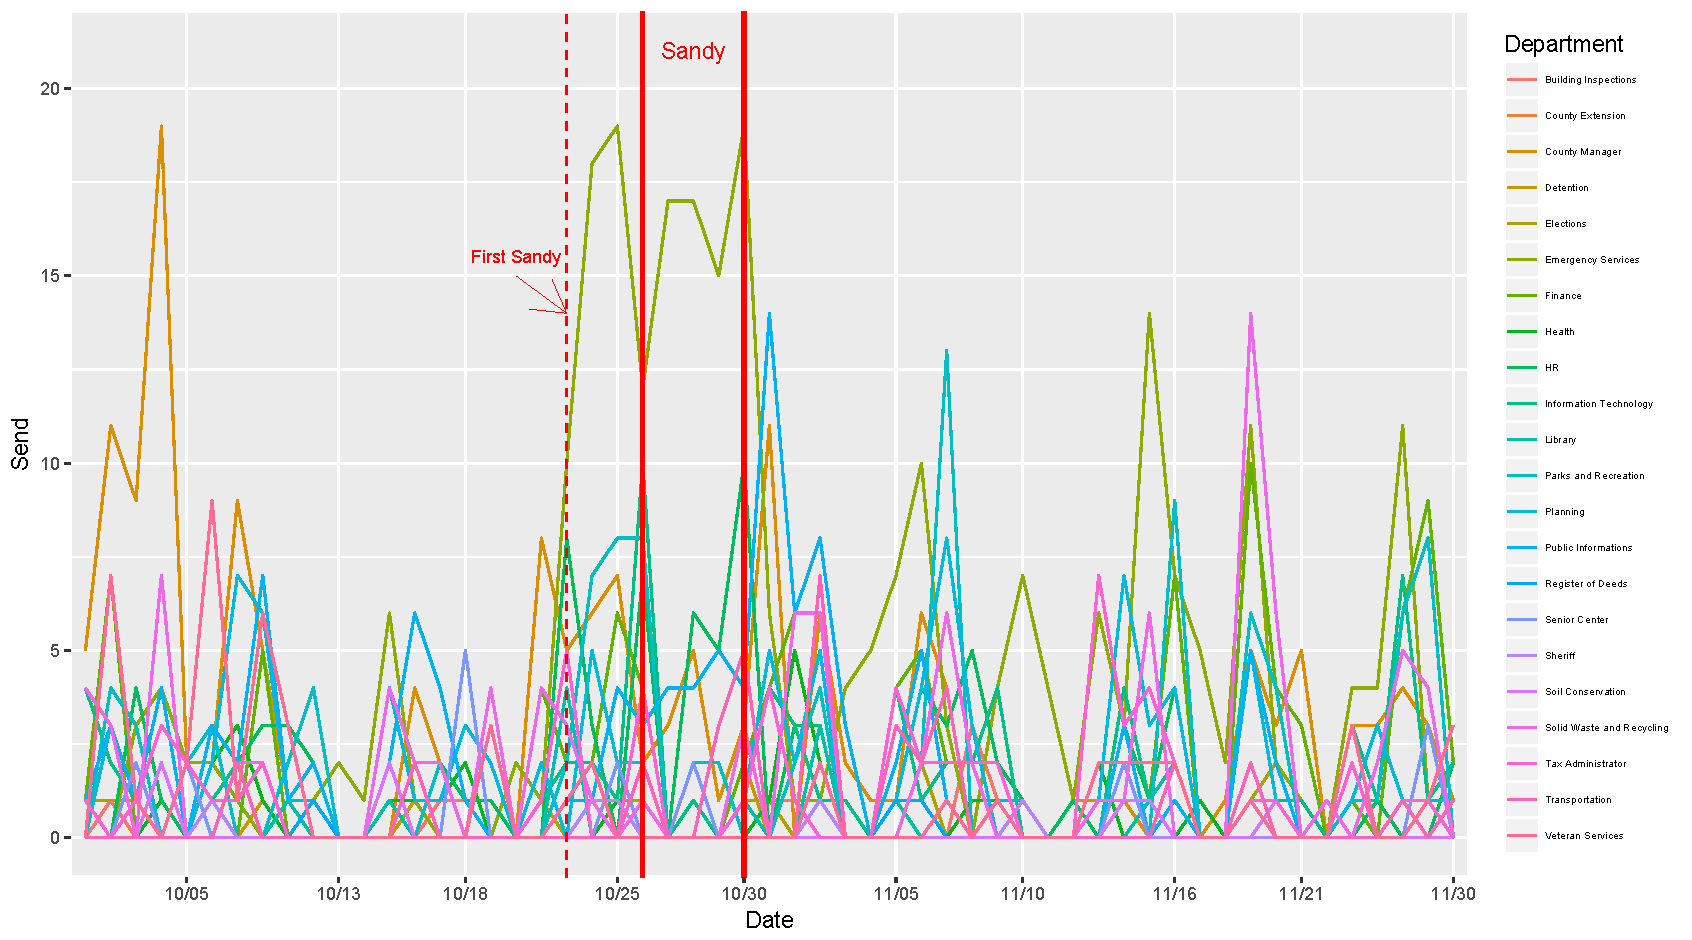
\includegraphics[width=0.5\textwidth]{Sendplot.pdf}	 	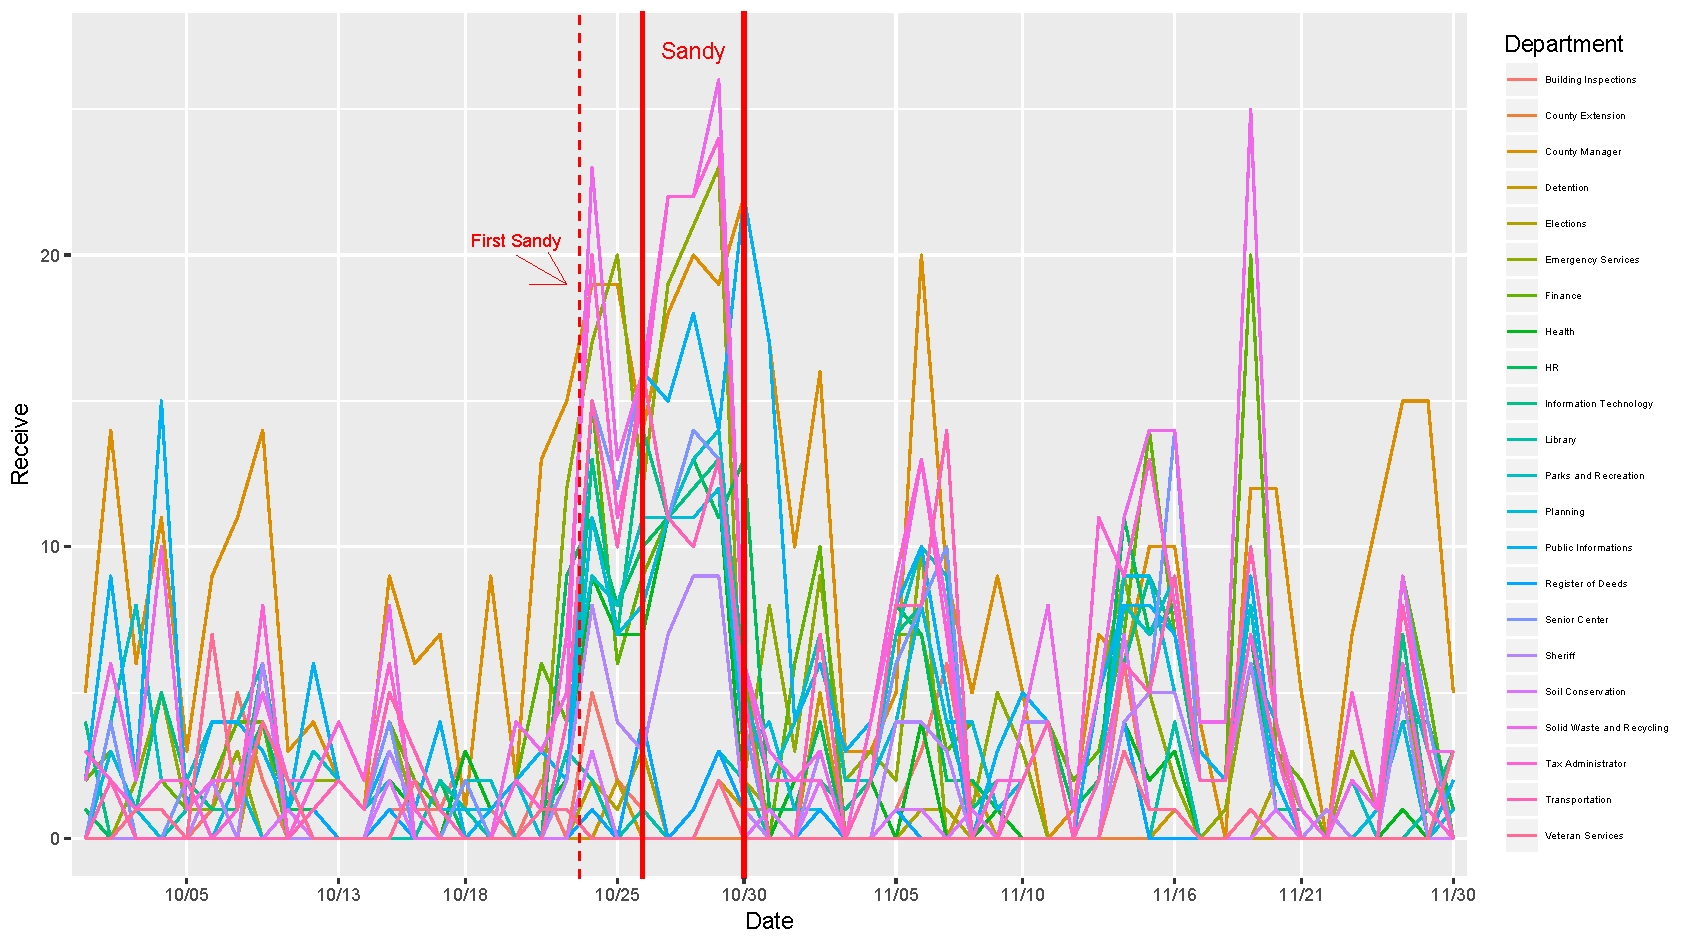
\includegraphics[width=0.5\textwidth]{Receiveplot.pdf}
	 \end{figure}	
\end{frame}

\begin{frame}{IPTM Result}
\end{frame}

\begin{frame}{Conclusion}
 \bni
 \item Joint modeling of ties (sender, receiver, time) and contents
 	\vspace{0.4cm}
 \item Allowance of multicast -- multiple senders and/or receivers
 	\vspace{0.4cm}
 \item Possible application to 
 \ei
\end{frame}
\end{document}